\documentclass[12pt,letterpaper]{article}
\usepackage{graphicx,textcomp}
\usepackage{natbib}
\usepackage{setspace}
\usepackage{fullpage}
\usepackage{color}
\usepackage[reqno]{amsmath}
\usepackage{amsthm}
\usepackage{fancyvrb}
\usepackage{amssymb,enumerate}
\usepackage[all]{xy}
\usepackage{endnotes}
\usepackage{lscape}
\newtheorem{com}{Comment}
\usepackage{float}
\usepackage{hyperref}
\newtheorem{lem} {Lemma}
\newtheorem{prop}{Proposition}
\newtheorem{thm}{Theorem}
\newtheorem{defn}{Definition}
\newtheorem{cor}{Corollary}
\newtheorem{obs}{Observation}
\usepackage[compact]{titlesec}
\usepackage{dcolumn}
\usepackage{tikz}
\usetikzlibrary{arrows}
\usepackage{multirow}
\usepackage{xcolor}
\newcolumntype{.}{D{.}{.}{-1}}
\newcolumntype{d}[1]{D{.}{.}{#1}}
\definecolor{light-gray}{gray}{0.65}
\usepackage{url}
\usepackage{listings}
\usepackage{color}
\usepackage{booktabs}
\usepackage[most]{tcolorbox}

\definecolor{codegreen}{rgb}{0,0.6,0}
\definecolor{codegray}{rgb}{0.5,0.5,0.5}
\definecolor{codepurple}{rgb}{0.58,0,0.82}
\definecolor{backcolour}{rgb}{0.95,0.95,0.92}

\lstdefinestyle{mystyle}{
	backgroundcolor=\color{backcolour},   
	commentstyle=\color{codegreen},
	keywordstyle=\color{magenta},
	numberstyle=\tiny\color{codegray},
	stringstyle=\color{codepurple},
	stepnumber=1,
	basicstyle=\footnotesize,
	breakatwhitespace=false,         
	breaklines=true,                 
	captionpos=b,                    
	keepspaces=true,                 
	numbers=left,                    
	numbersep=5pt,                  
	showspaces=false,                
	showstringspaces=false,
	showtabs=false,                  
	tabsize=2
}

\lstset{style=mystyle}
\newcommand{\Sref}[1]{Section~\ref{#1}}
\newtheorem{hyp}{Hypothesis}

\title{Problem Set 4}
\date{Due: April 12, 2024}
\author{Applied Stats II \\  Dan Zhang 23335541}


\begin{document}
	\maketitle
	\section*{Instructions}
	\begin{itemize}
	\item Please show your work! You may lose points by simply writing in the answer. If the problem requires you to execute commands in \texttt{R}, please include the code you used to get your answers. Please also include the \texttt{.R} file that contains your code. If you are not sure if work needs to be shown for a particular problem, please ask.
	\item Your homework should be submitted electronically on GitHub in \texttt{.pdf} form.
	\item This problem set is due before 23:59 on Friday April 12, 2024. No late assignments will be accepted.

	\end{itemize}

\newpage
\section*{Question 1}
\vspace{.25cm}
\noindent We're interested in modeling the historical causes of child mortality. We have data from 26855 children born in Skellefteå, Sweden from 1850 to 1884. Using the "child" dataset in the \texttt{eha} library, fit a Cox Proportional Hazard model using mother's age and infant's gender as covariates. Present and interpret the output.\vspace{.3cm}

\noindent Load data and check data structure.
\lstinputlisting[firstline=28,lastline=28,language=R]{PS04.R}

\begin{table}[htbp]
	\centering
	\caption{Structure of Child Data}
	\label{tab:Structure of Child Data}
	\begin{tabular}{@{}cccccccccc@{}}
		\toprule
		id & m.id & sex & socBranch & birthdate & enter & exit & event & illeg & m.age \\
		\midrule
		3 & 246606 & male & farming & 1853-05-23 & 0 & 15.000 & 0 & no & 35.009 \\
		42 & 377744 & male & farming & 1853-07-19 & 0 & 15.000 & 0 & no & 30.609 \\
		47 & 118277 & male & worker & 1861-11-17 & 0 & 15.000 & 0 & no & 29.320 \\
		54 & 715337 & male & farming & 1872-11-16 & 0 & 15.000 & 0 & no & 41.183 \\
		78 & 978617 & female & worker & 1855-07-19 & 0 & 0.559 & 1 & no & 42.138 \\
		102 & 282943 & male & farming & 1855-09-29 & 0 & 0.315 & 1 & no & 32.931 \\
		\bottomrule
	\end{tabular}
\end{table}

\noindent Use Surv() function to create a survive object and run  the Cox model.
\lstinputlisting[firstline=33,lastline=36,language=R]{PS04.R}
\begin{table}[!htbp]
	\centering
	\caption{The impact of maternal age and infant's gender on child survival}
	\label{tab:child_surv_analysis}
	\begin{tabular}{@{}lc@{}}
		\toprule
		& \textit{Dependent variable: child\_survival} \\ 
		\midrule
		m.age & 0.008$^{***}$ \\
		& (0.002) \\
		
		sexfemale & $-$0.082$^{***}$ \\
		& (0.027) \\
		\midrule
		Observations & 26,574 \\
		R$^{2}$ & 0.001 \\
		Max. Possible R$^{2}$ & 0.986 \\
		Log Likelihood & $-$56,503.480 \\
		Wald Test & 22.520$^{***}$ (df = 2) \\
		LR Test & 22.518$^{***}$ (df = 2) \\
		Score (Logrank) Test & 22.530$^{***}$ (df = 2) \\
		\bottomrule
	\end{tabular}
	\smallskip
	
	\textit{Note:} $^{*}$p$<$0.1; $^{**}$p$<$0.05; $^{***}$p$<$0.01
\end{table} 

\noindent Before interpreting the results, let's run a drop1() function to check covariables' contribution to the model.
\lstinputlisting[firstline=42,lastline=42,language=R]{PS04.R}

\begin{table}[!htbp]
	\centering
	\caption{Single Term Deletions from the Model Predicting Child Survival}
	\label{tab:single_term_deletions}
	\begin{tabular}{lcccc}
		\toprule
		Term & Df & AIC & LRT & Pr($>$Chi) \\
		\midrule
		\textit{none} & & 113011 & & \\
		\textit{m.age} & 1 & 113022 & 12.7946 & 0.0003476 *** \\
		\textit{sex} & 1 & 113018 & 9.4646 & 0.0020947 ** \\
		\bottomrule
	\end{tabular}
	
		\smallskip
	\textit{Note:} Significance codes: $^{***}$ p$<$0.001, $^{**}$ p$<$0.01, $^{*}$ p$<$0.05, $^{.}$ p$<$0.1
\end{table}

\noindent The model fits well. Have a look at the survival curve.

\lstinputlisting[firstline=50,lastline=55,language=R]{PS04.R}
\begin{figure}[htbp]
	\centering
	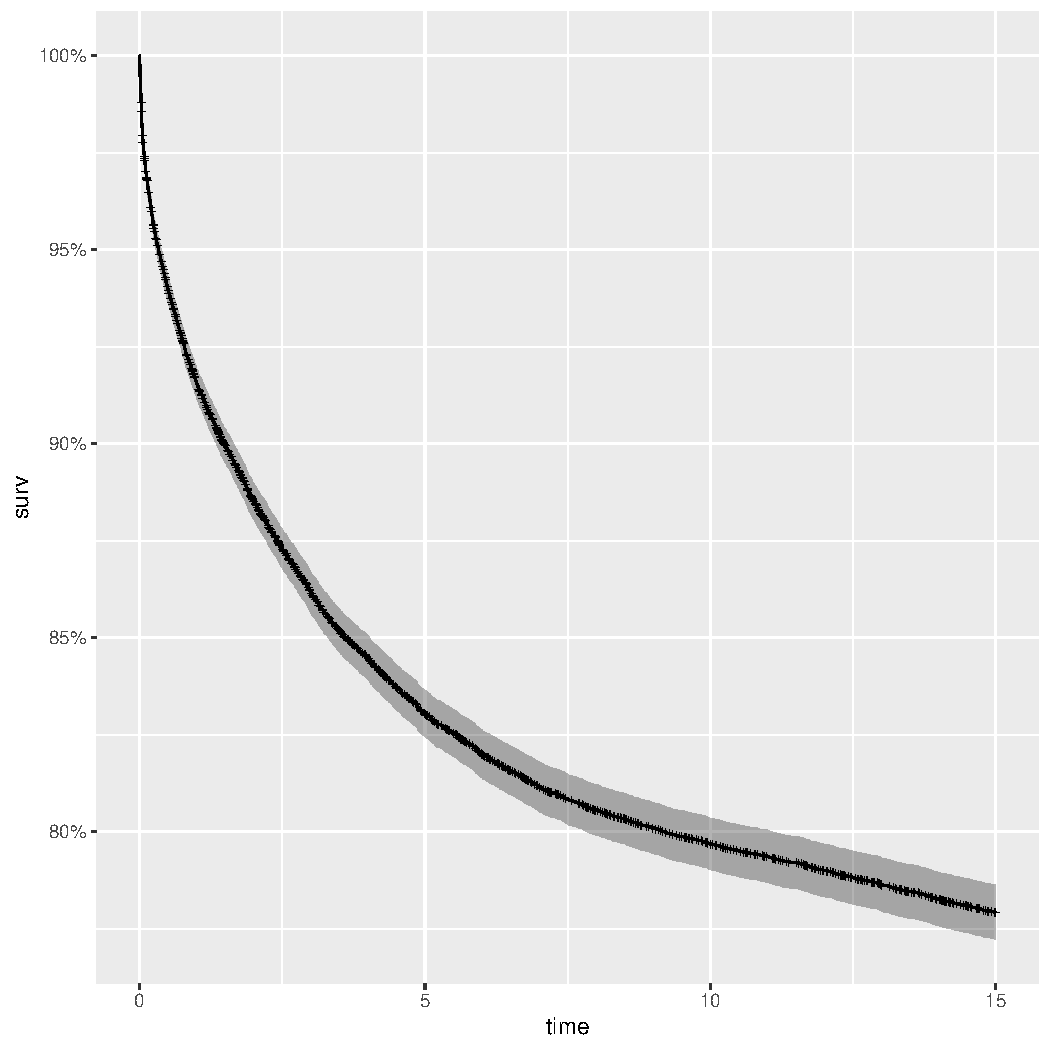
\includegraphics[width=0.6\linewidth]{Survial curve.pdf} 
	\caption{Survial curve} 
	\label{fig:Survial curve} 
\end{figure}


\noindent Calculate the exponential results of covariables to get the hazard ratio.
\lstinputlisting[firstline=48,lastline=48,language=R]{PS04.R}

\noindent Interpretation:
\begin{itemize}
	\item Coefficient of mother's age: The mother's age has a statistical significant positive impact on the infant's survival rate, with a coefficient of 0.008. For every one-year increase in maternal age, the log-hazard ratio of the infant's survival probability increases by an average of 0.008, holding other variables constant. The hazard ratio of female infant is 0.92 that of male infant, which means female infant are less likely to die, female deaths are 8\% lower.
	
	\item Coefficient of infant's gender: Compared with the reference group (male infant), the logarithm ratio of the survival rate of female children is reduced by 0.082 on average, holding other variables constant.
\end{itemize}
\noindent In conclusion, 

\noindent Run a interaction term with the covairables and check the model fit.

\lstinputlisting[firstline=58,lastline=63,language=R]{PS04.R}
	\begin{table}[h]
	\centering
		\caption{Single Term Deletions for interaction term model}
	\begin{tabular}{lcccc}
		\hline
		Term & Df & AIC & LRT & Pr($>$Chi) \\
		\hline
		None & - & 113013 & - & - \\
		m.age:sex & 1 & 113011 & 0.10623 & 0.7445 \\
		\hline
	\end{tabular}
	\label{table:single_term_deletions}
\end{table}

\noindent As p $>$ 0.05. This means that adding the m.age:sex interaction term did not bring statistically significant model improvements.


\end{document}